\fancyhead{}
\fancyfoot{}
\cfoot{\thepage}

\lhead{Método, enfoque e implementación}
% \chapter{Método}
\chapter{Método, enfoque e implementación}

\section{Método}

La investigación se centra en el desarrollo de un sistema de compras
inteligentes que utiliza datos históricos de ventas para optimizar la gestión
de insumos gastronómicos. La metodología implica la recopilación y análisis de
datos de ventas previas para identificar patrones y la aplicación de algoritmos
de aprendizaje automático para predecir futuras compras. Se evaluará la
precisión del sistema mediante métricas cuantitativas, y el alcance de la
investigación se concentra en un local gastronómico en Ciudad del Este,
detallando la recopilación de datos, la arquitectura del sistema y su capacidad
para generar predicciones de demanda basadas en el histórico de ventas.

% \begin{figure}[H]
%   \begin{center}
%     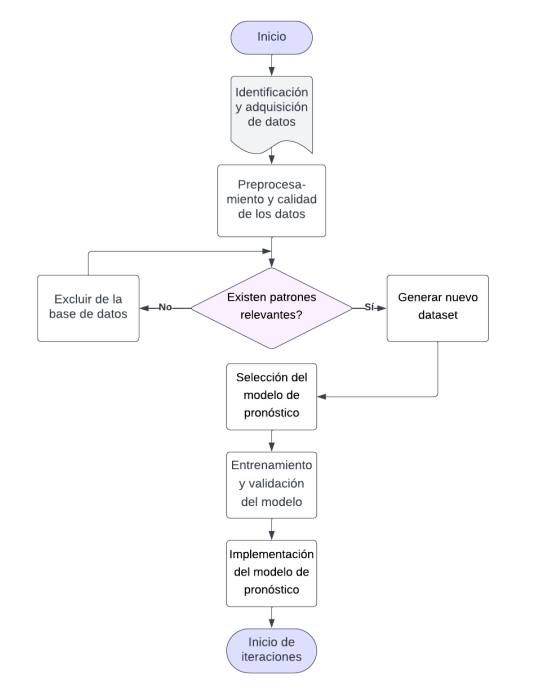
\includegraphics[scale=0.70]{./identificacion de patrones y tendencias.png}
%     \caption{Identificación de patrones y tendencias}
%     \label{fig:identificacion_patrones}
%   \end{center}
% \end{figure}

\section{Preprocesamiento de datos}
En esta sección, se describirán los métodos utilizados para llevar a cabo la
investigación sobre la predicción de compras a partir de un historial de ventas.

\subsection{Obtención de datos}
Los datos usados para generar el modelo fueron proporcionados por la empresa
gastronómica. La misma proporcionó el dataset para ser usado con fines
académicos, los datos presentan las ventas diarias para los diferentes
productos, cuenta con 6 meses de registro desde el 17 de abril del 2023 hasta el
15 de octubre del 2023.

Los datos originales suministrados están conformados por los siguientes
datasets:
\begin{itemize}
  \item productos.csv
  \item ventas.csv
\end{itemize}

Los datos vienen organizados en forma tabular, cada archivo presenta
información separada relacionada con los diferentes productos y el registro de
ventas histórico.

\vspace{1\baselineskip}
\textbf{productos.csv}

Estructura inicial de la tabla de productos (informacion de los 5 primeros
productos(Fig. \ref{fig:priemeros_5productos})).

\begin{figure}[H]
  \begin{center}
    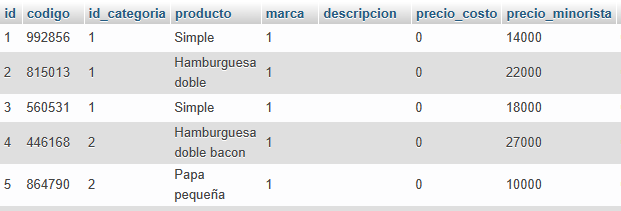
\includegraphics[scale=0.90]{./tabla_producto.png}
    \caption{Estructura inicial de la tabla productos.csv}
    \label{fig:priemeros_5productos}
  \end{center}
\end{figure}

\textbf{ventas.csv}

Estructura inicial de la tabla de ventas(con información de 6 registros (Fig.
\ref{fig:ventas_original})).

\begin{figure}[H]
  \begin{center}
    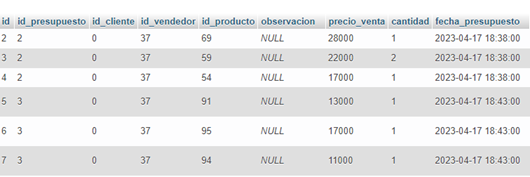
\includegraphics[scale=0.90]{./ventas_tabla.png}
    \caption{Estructura inicial de la tabla  ventas.csv}
    \label{fig:ventas_original}
  \end{center}
\end{figure}

%MODELADO
\subsection{Modelado de datos}
Antes de evaluar algún modelo, se debe llevar a cabo una limpieza de la
base de datos y acondicionamiento de las características finales en variables numéricas.

\vspace{1\baselineskip}
En el siguiente apartado se estara realizando el proceso de limpieza de los datos para la obtención de los parametros a utilizar.

\vspace{1\baselineskip}

Se obtuvieron las columnas necesarias de la tabla productos para el desarrolo
del proyecto, desde la base de datos MySQL herramienta utilizada para el
almacenamiento de los datos.

\vspace{1\baselineskip}
Hay varios sistemas de gestión de bases de datos gratuitos o de bajo coste disponibles, como MySQL, PostgreSQL o SQLite. Cuando comparas MySQL con otros sistemas de bases de datos, piense en lo que es más importante para usted. Características de rendimiento (como compatibilidad o extensiones de SQL),
soporte, condiciones de licencia y precio, todo son factores a tener en cuenta \cite{dubois2013mysql}.

Dadas estas consideraciones, MySQL tiene muchas cualidades atractivas:

\begin{itemize}
  \item Velocidad.
  \item Facilidad de uso.
  \item Soporte de lenguaje de consulta. MySQL entiende SQL (consulta estructurada
        Language), el lenguaje estándar elegido para todos los sistemas de bases de
        datos modernos.
  \item Capacidad. El servidor MySQL es multihilo, lo que permite que muchos clientes se conecten a él al mismo tiempo. Cada cliente puede usar múltiples bases de datos simultáneamente.
  \item Conectividad y seguridad. MySQL es completamente en red, y las bases de datos se pueden acceder desde cualquier lugar de Internet, lo que le permite compartir sus datos con cualquier persona, en cualquier lugar.
  \item Portabilidad. MySQL se ejecuta en muchas variedades de Unix y Linux, así como en otros sistemas como Windows.
  \item Disponibilidad y costos. MySQL es un proyecto de código abierto disponible bajo múltiples términos de licencia

\end{itemize}



La siguiente consulta SQL selecciona las columnas \texttt{id} y
\texttt{producto} de la tabla \texttt{productos}, donde la columna
\texttt{anulado} tiene un valor nulo:
\begin{center}
  \begin{verbatim}
    SELECT id, producto
    FROM productos
    WHERE anulado IS NULL;
  \end{verbatim}
\end{center}
\begin{figure}[H]
  \begin{center}
    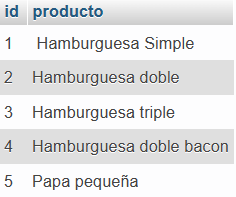
\includegraphics[scale=0.90]{./primeros_5productos.png}
    \caption{Datos de la tabla productos(Los primeros 5 productos)}
    \label{fig:priemeros_5productos}
  \end{center}
\end{figure}

En la tabla \ref{tab:productos} se muestra una descripción de cada una de las
columnas de productos.

\begin{table}[H]

  \begin{tabular}{|c|l|}  % Usamos "l" para alinear a la izquierda
    \hline
    \rowcolor{gray!50} \textbf{Columna} & \textbf{Descripción}                     \\
    \hline
    id                                  & el id del producto (identificador unico) \\
    producto                            & el nombre del producto                   \\
    \hline
  \end{tabular}
  \centering
  \caption{ Descripción de datos de la tabla de productos}
  \label{tab:productos} % Asigna una etiqueta a la tabla
\end{table}

La consulta SQL a continuación selecciona las columnas \texttt{id\_producto},
\texttt{cantidad}, y \texttt{fecha\_venta} de la tabla \texttt{ventas} para las
transacciones que tuvieron lugar en el período desde el 17 de abril de 2023
hasta el 15 de octubre de 2023 donde la columna \texttt{anulado} tiene un valor
nulo (Figura:\ref{fig:fecha_venta}):

\begin{verbatim}
  SELECT id_producto, cantidad, fecha_venta
  FROM ventas
  WHERE fecha_venta BETWEEN '2023-04-17' AND '2023-10-15'
  AND anulado IS NUL;
\end{verbatim}
\begin{figure}[H]
  \begin{center}
    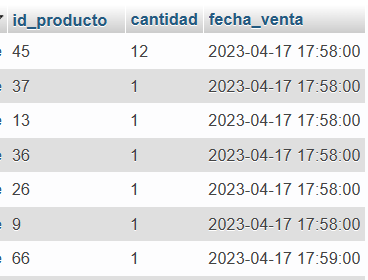
\includegraphics[scale=0.90]{./ventas_fecha.png}
    \caption{Datos de la tabla ventas}
    \label{fig:fecha_venta}
  \end{center}
\end{figure}

En la tabla \ref{tab:ventas_fechas} se muestra una descripción de cada una de
las columnas de productos.

\begin{table}[H]

  \begin{tabular}{|c|l|}  % Usamos "l" para alinear a la izquierda
    \hline
    \rowcolor{gray!50} \textbf{Columna} & \textbf{Descripción}                     \\
    \hline
    id\_producto                        & el id del producto (identificador unico) \\
    catidad                             & cantidad de venta                        \\
    fecha\_venta                        & fecha de la venta                        \\
    \hline
  \end{tabular}
  \centering
  \caption{ Descripción de datos de la tabla ventas}
  \label{tab:ventas_fechas} % Asigna una etiqueta a la tabla
\end{table}

%ESCALADO

\subsection{Escalado de datos}

El escalado de datos es un proceso esencial en el análisis de datos y la estadística que ajusta los valores de las variables para que compartan una misma escala o propiedades específicas.

\vspace{1\baselineskip}
La consulta SQL se enfoca en el escalado de datos de ventas de productos durante un periodo del 17 de abril al 15 de octubre, excluyendo ventas anuladas. La consulta agrupa los resultados por producto y fecha de venta, permitiendo así obtener una visión escalada de la cantidad total vendida de cada producto a lo largo del tiempo, lo que facilita la identificación de tendencias y patrones en las ventas.

\begin{verbatim}
  SELECT id_producto, SUM(cantidad) AS Cantidad, fecha_venta
  FROM ventas
  WHERE fecha_venta BETWEEN '2023-04-17' AND '2023-10-15'
  AND anulado IS NULL
  GROUP BY id_producto, fecha_venta;
\end{verbatim}

\begin{figure}[H]
  \begin{center}
    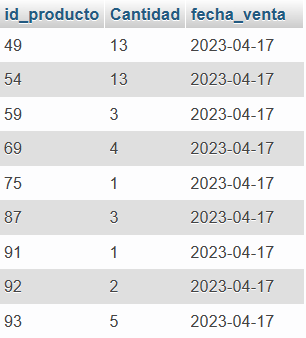
\includegraphics[scale=0.90]{./escalado.png}
    \caption{Datos escalados(muestra de la tabla ventas)}
    \label{fig:escalado}
  \end{center}
\end{figure}

\begin{table}[H]

  \begin{tabular}{|c|l|}  % Usamos "l" para alinear a la izquierda
    \hline
    \rowcolor{gray!50} \textbf{Columna} & \textbf{Descripción}                               \\
    \hline
    id\_producto                        & el id del producto                                 \\
    catidad                             & suma de la cantidad de ventas por fecha y producto \\
    fecha\_venta                        & fecha de la venta                                  \\
    \hline
  \end{tabular}
  \centering
  \caption{ Descripción de datos escalados de la tabla ventas }
  \label{tab:tabla_scalada} % Asigna una etiqueta a la tabla
\end{table}

%ANALISIS DE LOS DATOS
\subsection{Análisis de los datos }
El objetivo principal de esta etapa es explorar y comprender en profundidad los datos, lo que resulta fundamental para una sólida preparación y análisis de los mismos. Esta comprensión más profunda del problema de negocio nos permitirá seleccionar modelos de predicción y tomar decisiones más fundamentadas. Durante el proceso de limpieza y preparación de los datos, se han identificado características relevantes que proporcionarán información valiosa para las fases posteriores del análisis y la toma de decisiones.

\vspace{1\baselineskip}
Como se observa(Figura: \ref{fig:fecha_venta}), la base de datos de entrenamiento es limitada en términos de variables disponibles. En este escenario, se ha seleccionado exclusivamente la fecha como variable de entrada y se ha focalizado en un producto específico, en este caso, la“Hamburguesa simple” con id\_producto 49, debido a su alta demanda. Se han recopilado 182 registros ya agrupados por día, lo que equivale a 182 días de datos. El propósito de este enfoque es analizar el comportamiento de las ventas de dicho
producto en relación al tiempo y buscar patrones que puedan mejorar la precisión del modelo de predicción.

\begin{figure}[H]
  \begin{center}
    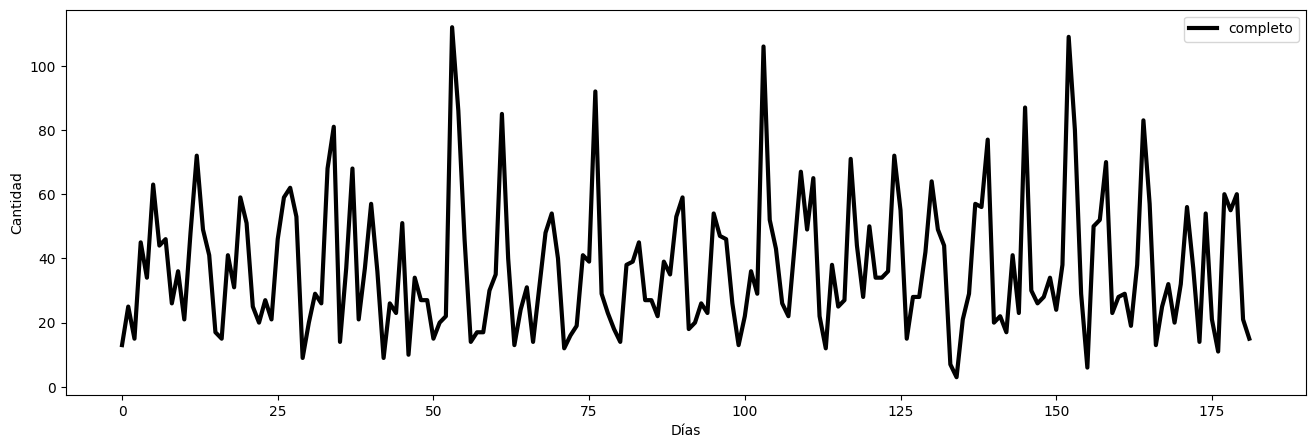
\includegraphics[scale=0.40]{./serie_normal_completa.png}
    \caption{Serie temporal de las ventas totales por día}
    \label{fig:serie_completa}
  \end{center}
\end{figure}

%   En la tabla \ref{tab:ventas} se muestra una descripción de cada una de las columnas de ventas.
%   

% \section{Enfoque}
% El desarrollo de un sistema de compras inteligentes que utiliza un histórico de ventas como fuente principal de información. El objetivo principal es optimizar la gestión de insumos gastronómicos.

% \begin{itemize}
% \item Recopilación y análisis de datos cuantitativos de ventas históricas para desarrollar un modelo predictivo. Esto abarcaría la identificación de patrones de ventas, el uso de algoritmos de aprendizaje automático para predecir futuras compras y la evaluación de la precisión del sistema. 
% \item Aplicación de métricas cuantitativas para evaluar el rendimiento del sistema en términos de eficiencia, impacto en las ventas y beneficios para la entidad objeto de estudio.

% \end{itemize}

% \section{Alcance de la investigación cuantitativa}
% El alcance de esta investigación descriptiva se enfoca en proporcionar una visión detallada y exhaustiva de la aplicación de un sistema inteligente de gestión de compras basado en el histórico de ventas en un local gastronómico ubicado en Ciudad del Este. 
% Se describirá el proceso de recopilación de datos históricos de ventas, incluyendo la fuente de los datos, el periodo de tiempo cubierto y la naturaleza de la información registrada.
% Se proporcionará una descripción completa de cómo opera el sistema inteligente computarizado, incluyendo su arquitectura, algoritmos de pronóstico, y la forma en que utiliza los datos históricos para generar predicciones de demanda.

%VARIABLES DE ENTRADA Y SALIDA
\subsection{Definición de las variables de entrada y salida}

Se han considerado estas variables como variables de entrada debido a que, a través del análisis de la serie temporal de ventas, se han identificado patrones y tendencias significativas que impactan en las ventas del producto.

\vspace{1\baselineskip}
El mes, el día del mes, el día de la semana, la presencia de días festivos y la estación del año influyen directamente en el comportamiento de las ventas. 

\vspace{1\baselineskip}
El promedio de venta mensual varía, lo que indica una estacionalidad en la demanda. Las ventas tienden a aumentar hacia el final e inicio del mes, posiblemente relacionado con el ciclo de pagos de los consumidores. La influencia de los días de la semana sugiere que los fines de semana son momentos clave para las ventas. La presencia de días festivos genera picos en las ventas, lo que puede estar vinculado a la celebración y al aumento de la
demanda en esas fechas. Por último, la estación del año también desencadena cambios en las ventas, con un aumento en verano, lo que respalda la necesidad de considerar esta variable en el modelo para una predicción más precisa.

\vspace{1\baselineskip} Teniendo todas estas informaciones, se procede a la
conversión de estas características en variables de entrada y salida para el
aprendizaje del modelo, y se asegura de que estén representadas en formato
numérico.

\begin{table}[H]
  \begin{tabular}{|c|l|l|}  % Usamos "l" para alinear a la izquierda
    \hline
    \rowcolor{gray!50} \textbf{Columna} & \textbf{Descripción}              & \textbf{Dato numerico} \\
    \hline
    mes                                 & variable mes Rango                & 1-12                   \\
    dia                                 & variable dias del mes Rango       & 1-31                   \\
    dia\_semana                         & variable dia de la semana Rango   & 0-6                    \\
    dia\_festivo                        & variable dia festivo Rango        & 0-1                    \\
    estacion                            & variable estaciones del año Rango & 0-3                    \\
    \hline
  \end{tabular}
  \centering
  \caption{ Variables de entrada}
  \label{tab:variables_de _entrada} % Asigna una etiqueta a la tabla
\end{table}

La siguiente consulta SQL realiza un análisis de ventas de un producto con
id\_producto igual a 49. Agrupa los datos por fecha de venta y calcula diversas
métricas relacionadas con la fecha, como el mes, el día, el día de la semana y
si la fecha es un día festivo. También determina la estación correspondiente a
cada fecha y agrega información sobre la cantidad total de ventas y la suma de
las cantidades vendidas para cada día. En resumen, esta consulta proporciona un
resumen detallado de las ventas del producto 49, organizado por fecha y con
métricas relacionadas con la fecha para su posterior utilización.

\begin{verbatim}
  SELECT MONTH(fecha_venta) AS mes, 
  DAY(fecha_venta) AS dia, 
  DAYOFWEEK(fecha_venta) AS dia_semana, 
  IFNULL((SELECT 1 FROM dias_festivos df 
  WHERE CAST(v.fecha_venta AS date)=df.fecha),0) AS dia_festivo, 
  (SELECT estacion FROM estaciones e 
  WHERE cast(v.fecha_venta AS date) 
  BETWEEN e.fecha_inicio AND e.fecha_fin) AS estacion,
  COUNT(id_venta) AS cantidad_ventas, 
  SUM(v.cantidad) AS cantidad 
  FROM ventas v 
  WHERE id_producto = 49 
  GROUP BY CAST(fecha_venta AS date)
\end{verbatim}

% Tabla (\ref{fig:tabla_resultante})resultante en formato .csv con el exportador
% de MySQL
\begin{figure}[H]
  \begin{center}
    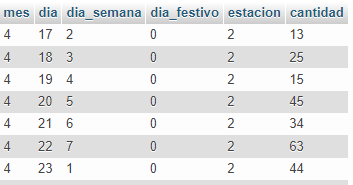
\includegraphics[scale=0.90]{./tabla_resultante.png}
    \caption{Tabla resultante con las variables de entrada}
    \label{fig:tabla_resultante}
  \end{center}
\end{figure}

%LECTURA Y ESCALADO

\subsection{Lectura y escalado del dataset en Python}
% En este trabajo se realiza todo el proceso en el software Python.

% \vspace{1\baselineskip}
La elección de Python como lenguaje de programación se fundamenta en su destacado uso en el campo de la inteligencia artificial, respaldado por una amplia gama de bibliotecas y una comunidad activa\cite{mirjalili2020python}. En cuanto al entorno de pruebas, se ha optado por Google Colab debido a su facilidad de uso y su gratuidad, lo que lo convierte en una opción conveniente para el desarrollo y la prueba de modelos de inteligencia artificial.

\vspace{1\baselineskip}
Los datos se preparan de manera similar tanto para las pruebas en el modelo de regresión lineal como para el modelo LSTM, lo que implica el proceso de escalado y la división en variables de entrada y salida (Figura: \ref{fig:lectura_escalado}).

% En Python, se emplea la biblioteca pandas para la lectura de archivos CSV, y para el escalado, se recurre al MinMaxScaler de la librería sklearn .

\vspace{1\baselineskip}
Python es un lenguaje muy maduro, versátil, y se puede utilizar como una plataforma specífica para el Data Science, gracias a su gran ecosistema de librerías científicas y a su comunidad, que es muy activa \cite{chilet2023elaboracion}.

\vspace{1\baselineskip}
En este proyecto se emplean algunas de ellas que nos facilitaran el proceso a la hora de realizar diferentes
funciones.

\begin{itemize}
  \item \textbf{NumPy:} Ofrece una amplia gama de funciones matemáticas y herramientas para trabajar con datos numéricos, como generadores de números aleatorios, rutinas de álgebra lineal, transformadas de Fourier y más. Esto hace que NumPy sea una biblioteca esencial en aplicaciones científicas y de análisis de datos, ya que proporciona las herramientas necesarias para realizar cálculos numéricos de manera eficiente y rápida \cite{numpy-website}. 
  \item \textbf{Pandas:} Es una biblioteca de Python ampliamente utilizada en la manipulación y análisis de datos. Ofrece un objeto eficiente llamado DataFrame para trabajar con datos tabulares, facilitando la lectura y escritura de datos desde diversas fuentes \cite{pandas-website}. 
  \item \textbf{Matplotlib:} Esta librería de software gráfico permite la generación de gráficos en dos dimensiones, a partir de datos contenidos en listas o arrays. Junto con Pandas han sido las dos librerías de Python que más se han empleado en el proyecto para el tratamiento de los datos \cite{MatplotlibWebsite}.
  \item \textbf{TensorFlow:} Es una potente biblioteca de aprendizaje automático que permite a los desarrolladores y científicos de datos diseñar, entrenar y desplegar modelos de inteligencia artificial en una amplia gama de aplicaciones. \cite{tensorflow-website}.
  \item  \textbf{Keras:} Es una biblioteca de alto nivel para construir y entrenar redes neuronales en Python. Ofrece una interfaz sencilla y modular, siendo valiosa para desarrolladores y científicos de datos. Aunque es compatible con varios backends, TensorFlow se utiliza comúnmente en combinación con Keras para proyectos de aprendizaje profundo \cite{keras-doc}.
  \item \textbf{Scikit-Learn:} Es una librería de aprendizaje automático que contiene herramientas para la predicción de series temporales, incluyendo modelos de regresión y redes neuronales \cite{sepulveda2023analisis}.
\end{itemize}

Además de estas librerías, existen otras herramientas que se pueden utilizar en Python para la predicción de series temporales, como Prophet, que es una librería para el análisis y la predicción de series temporales con estacionalidad.

\begin{figure}[H]
  \begin{center}
    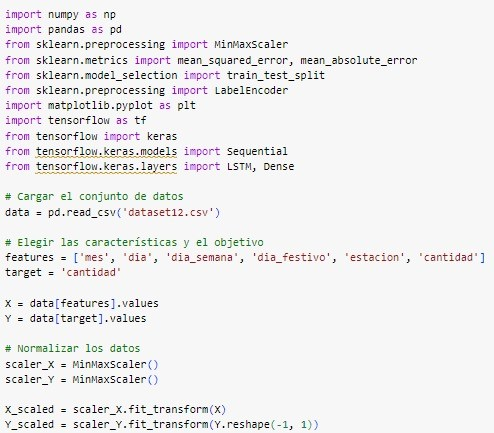
\includegraphics[scale=0.90]{./lectura_escalado.jpg}
    \caption{Codigo de lectura y escalado del dataset en Python}
    \label{fig:lectura_escalado}
  \end{center}
\end{figure}

El gráfico de violín es una herramienta valiosa en el análisis de datos y, en particular, en el contexto de escalado de datos, ya que proporciona una representación más completa y detallada de las distribuciones, lo que puede ayudar a comprender mejor la estructura de los datos y evaluar los efectos del escalado en la distribución de datos.

\vspace{1\baselineskip}
En el grafico \ref{fig:grafico_violin} se puede observar que todas las variables de entrada estan escaladas entre 0 y 1 incluyendo el set train,validación y test.
\begin{figure}[H]
  \begin{center}
    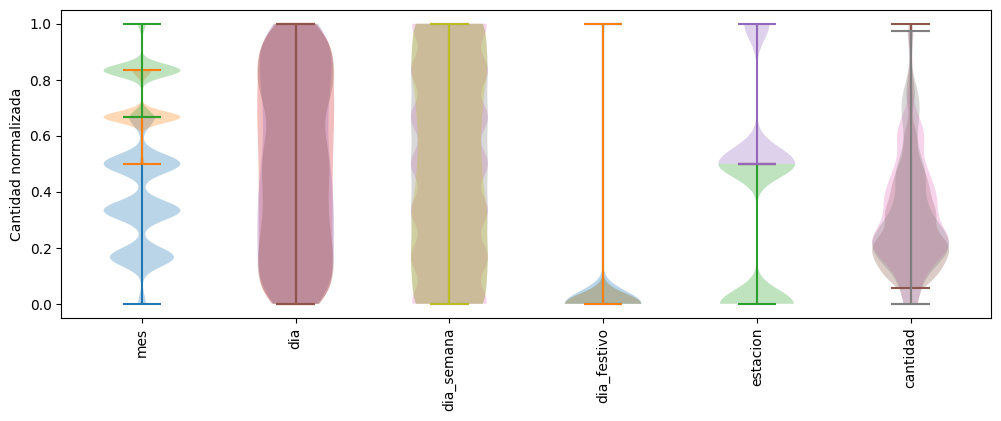
\includegraphics[scale=0.50]{./grafico tipo violin de escalado.png}
    \caption{Grafico en violín incluyendo los tres set train, validación y test}
    \label{fig:grafico_violin}
  \end{center}
\end{figure}

En el grafico \ref{fig:grafico_violin_salida} se puede observar que los datos
de salida también estén escaladas correctamente.
\begin{figure}[H]
  \begin{center}
    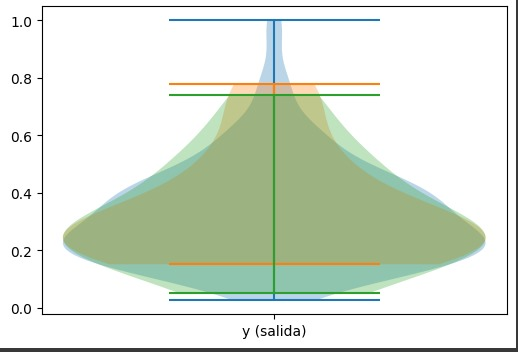
\includegraphics[scale=0.50]{./grafico_violin_salida.jpg}
    \caption{Gráfico en violín de los datos de salida escaladas}
    \label{fig:grafico_violin_salida}
  \end{center}
\end{figure}

%DISTRIBUCION DE LOS DATOS
\subsection{Distribución del conjunto de datos}

En el proceso de entrenamiento, es fundamental dividir el conjunto de datos en
tres conjuntos distintos:

\begin{itemize}
  \item \textbf{Conjunto de Entrenamiento (Train)}: Este conjunto se utiliza para entrenar el modelo, lo que significa que el modelo aprenderá de estos datos durante el proceso de entrenamiento.

  \item \textbf{Conjunto de Validación (Val)}: El conjunto de validación se emplea para evaluar si el modelo está sobreajustando los datos de entrenamiento. Ayuda a ajustar parámetros y prevenir el sobreajuste.

  \item \textbf{Conjunto de Prueba (Test)}: Este conjunto no se utiliza durante el entrenamiento del modelo y contiene datos con valores desconocidos. Se utiliza al final para evaluar la precisión del modelo en un entorno real, ya que no ha tenido acceso a estos datos previamente.
\end{itemize}

Se toma inicialmente 70\% train, 15\% val y 15\% test, como valores comúnmente
utilizados para estos casos.
\begin{figure}[H]
  \begin{center}
    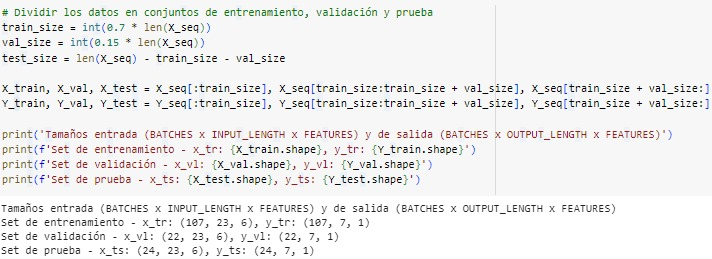
\includegraphics[scale=0.75]{./divisionde _datos.jpg}
    \caption{Codigo de distribución de los datos.}
    \label{fig:distribucion_algoritmo}
  \end{center}
\end{figure}

\begin{figure}[H]
  \begin{center}
    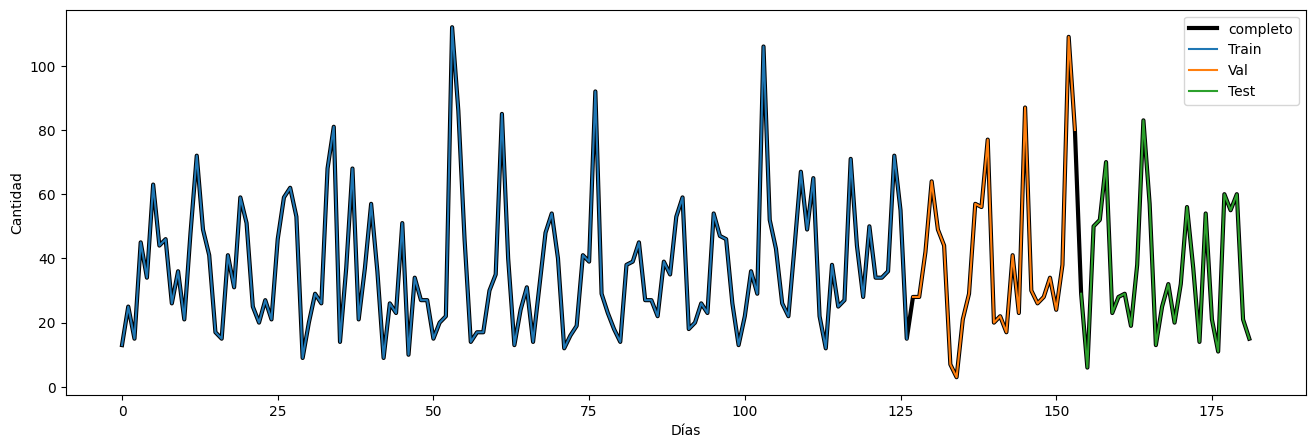
\includegraphics[scale=0.40]{./serie_normal_dividida.png}
    \caption{Distribución de los datos, ventas totales por día.}
    \label{fig:distribucion_datos}
  \end{center}
\end{figure}

%APLICACION Y COMPARACION
\section{Modelos de predicción}
Finalmente, todo el desarrollo del trabajo que se describirá a continuación referente al tratamiento de datos, entrenamiento de los modelos, evaluación de las métricas y su representación gráfica se ejecutará usando Python con el fin de aprovechar su uso por medio
de librerías como Numpy, Matplotlib, Pandas, Scikit-Learn el cual facilitará la solución de los requerimientos necesarios en cada punto del proceso.

%REGRESION LINEAL
\subsection{Modelo de Regresión lineal}


Para la implementación de regresión lineal, se ha optado por utilizar el
SGDRegressor de la biblioteca sklearn. En lo que respecta a la elección de
hiperparámetros, se han seleccionado valores comunes para un modelo de
regresión lineal implementado a través del algoritmo de Descenso de Gradiente Estocástico (SGD).

Estos parametros son los siguientes:

\begin{itemize}
  \item \textbf{loss}: Es una función de pérdida en la regresión lineal que mide la diferencia entre las predicciones del modelo y los valores reales. Su objetivo es minimizar esta discrepancia para encontrar la mejor línea de ajuste a los datos.

  \item \textbf{penalty}: Se ha especificado la regularización Ridge, que es una técnica comúnmente utilizada para abordar problemas de regresión. La regularización Ridge ayuda a prevenir el sobreajuste incorporando un término de penalización en la función de pérdida.

  \item \textbf{alpha}: El hiperparámetro de regularización controla la intensidad de la regularización.

  \item \textbf{max\_iter}: Se ha establecido el número máximo de iteraciones permitidas para el descenso de gradiente.

  \item \textbf{tol}: La tolerancia se utiliza para determinar cuándo se ha alcanzado la convergencia.

  \item \textbf{learning\_rate}: Se ha configurado la tasa de aprendizaje como constante a lo largo del proceso de entrenamiento.
\end{itemize}

\textbf{Fase de entrenamiento:}

En esta fase se tiene una cantidad enorme de datos, de la cual se separa una
parte para entrenar al algoritmo y darle toda esta información para que
encuentre los patrones necesarios y después pueda hacer predicciones.

El modelo se entrena con los datos de entrenamiento (X\_train, Y\_train)
utilizando el método .fit(). El modelo ajusta la línea de regresión a estos
datos para realizar predicciones (Figura \ref{fig:estructura_lineal_cap3}).

\vspace{1\baselineskip}
\textbf{Fase de prueba:}

El resto de los datos que quedan, se van a usar para hacer las pruebas. Así le
podemos hacer preguntas al algoritmo y evaluar si las respuestas están bien o
mal, y saber si está aprendiendo o no. Si vemos que no coinciden los datos,
tendremos que agregar más datos o cambiar el método que estamos utilizando.
Pero si se observa que hay entre un 80\% a 90\% de respuestas correctas,
podemos decir que hay un buen grado de aprendizaje y poder utilizar ese
algoritmo.

\vspace{1\baselineskip}
\textbf{Realizar Predicciones en Conjuntos de Datos: (Figura \ref{fig:estructura_lineal_cap3})}

\begin{itemize}
  \item Se realizan predicciones en tres conjuntos de datos diferentes: entrenamiento,
        validación y prueba.
  \item Para cada conjunto, se utiliza el modelo para predecir los valores de la
        variable objetivo.
  \item Las predicciones se almacenan en las variables $Y_{\text{train\_pred}}$,
        $Y_{\text{val\_pred}}$ y $Y_{\text{test\_pred}}$, respectivamente.
  \item Se utiliza el método \texttt{.ravel()} para asegurarse de que las predicciones
        tengan la forma correcta.
\end{itemize}

\begin{figure}[H]
  \begin{center}
    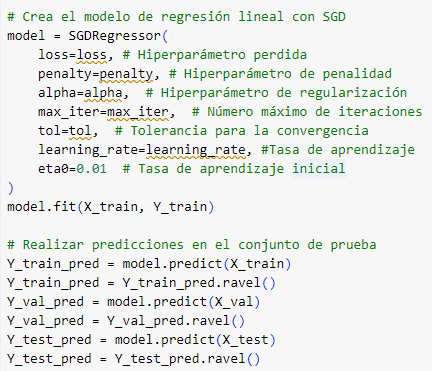
\includegraphics[scale=0.90]{./arquitectura REGRESION LINEAL.png}
    \caption{Codigo de la estructura de regresión lineal.}
    \label{fig:estructura_lineal_cap3}
  \end{center}
\end{figure}

\textbf{Fase de validacion:}

El proceso de validación implica calcular y comparar estas métricas utilizando
los datos de validación y prueba. Un buen modelo de regresión lineal debería
tener valores bajos de MSE y MAE, así como un alto valor de R² en ambos
conjuntos de datos, lo que indica que las predicciones se ajustan bien a los
valores reales. La validación es esencial para evaluar el rendimiento del
modelo en datos no vistos y garantizar su capacidad de generalización.

% \vspace{1\baselineskip}
% \textbf{Matplotlib} es una biblioteca completa para crear visualizaciones estáticas, animadas e interactivas en Python. Matplotlib hace que las cosas fáciles sean fáciles y las difíciles posibles\cite{MatplotlibWebsite}.

\begin{figure}[H]
  \begin{center}
    \includegraphics[scale=0.60]{./Grafico de predicciones con regresión.png}
    \caption{Grafico de lineas con Matplotlib.}
    \label{fig:prediccion_regresion_cap3}
  \end{center}
\end{figure}

%LSTM
\subsection{Modelo LSTM}

La red neuronal LSTM se modela con ayuda de la librería keras, es una librerıa
de codigo abierto de redes neuronales, que se implementa sobre otros frameworks
de aprendizaje automático como Tensorflow, CNTK o theano. Aparecio en 2015 y
fue creada por Fran¸cois Chollet. Tal y como se menciona en su documentación
\cite{keras-doc}, Keras se guía por cuatro principios. Ser amigable para el
usuario, modular, fácilmente extensible e implementada en python.

\vspace{1\baselineskip}
Al configurar una red neuronal LSTM, es común considerar varios hiperparámetros
clave (Codigo \ref{fig:desenpeño}):

\begin{itemize}
  \item \textbf{Unidades de LSTM:} Por lo general, se comienza con un número moderado de unidades en las capas LSTM, como 64 o 128. Aumentar el número de unidades puede ayudar a capturar patrones más complejos, aunque conlleva un mayor riesgo de sobreajuste.

  \item \textbf{Número de capas LSTM:} Para problemas más complejos, es posible agregar capas adicionales. Las arquitecturas con dos capas LSTM son comunes y funcionan bien en muchas aplicaciones.

  \item \textbf{Función de Activación:} Para las capas LSTM, la función de activación predeterminada suele ser “tanh”. No obstante, se pueden explorar otras funciones como “relu” o “sigmoid” según las necesidades del problema.

  \item \textbf{Función de Pérdida:} En problemas de regresión, es común utilizar el "mean squared error" (MSE) como función de pérdida. No obstante, la elección puede variar según el problema en particular.

  \item \textbf{Optimizador:} El “Adam” es un optimizador sólido y ampliamente utilizado en problemas de aprendizaje profundo. Aunque existen otras opciones como “RMSprop,” la elección depende en gran medida del contexto.

  \item \textbf{Tasa de Aprendizaje:} La tasa de aprendizaje es un hiperparámetro crucial. Por lo general, se comienza con un valor bajo, como 0.001, y se ajusta según la convergencia del modelo.

  \item \textbf{Dropout:} La técnica de dropout, aplicada en un porcentaje determinado de neuronas durante el entrenamiento, puede ayudar a prevenir el sobreajuste. Se recomienda iniciar con un valor del 20\% y ajustar según las necesidades del problema.
\end{itemize}

Es importante tener en cuenta que la elección de estos hiperparámetros puede
depender en gran medida del problema específico y requiere experimentación para
encontrar la configuración óptima.

\vspace{1\baselineskip}
\textbf{Diseño y Entrenamiento del Modelo LSTM:}
\begin{itemize}
  \item Diseña un modelo LSTM.
  \item Compila el modelo con función de pérdida y optimizador.
  \item Entrena el modelo con datos de entrenamiento.
\end{itemize}

\begin{figure}[H]
  \begin{center}
    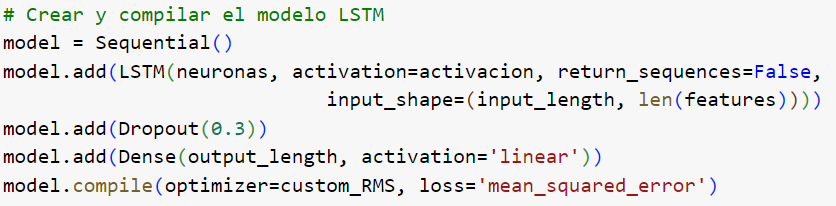
\includegraphics[scale=0.60]{./arquitectura LSTM.png}
    \caption{Codigo de la estructura del LSTM.}
    \label{fig:estructura_lstm}
  \end{center}
\end{figure}

\textbf{Validación del Modelo:}

\vspace{1\baselineskip}

Evalúa el rendimiento del modelo con datos de prueba.

\vspace{1\baselineskip}

\textbf{Conjunto de prueba 1:}
\begin{itemize}
  \item División del conjunto de datos: 70\% train, 20\% validation, 10\% test
  \item Optimizador: Adam
  \item Pérdida: Mean Squared Error (mean\_squared\_error)
  \item Épocas: 200
  \item Tamaño de lotes: 30
  \item Estructura de red: 1 capa oculta con 64 neuronas
  \item Función de activación: Linear
\end{itemize}

\vspace{1\baselineskip}

\begin{figure}[H]
  \begin{center}
    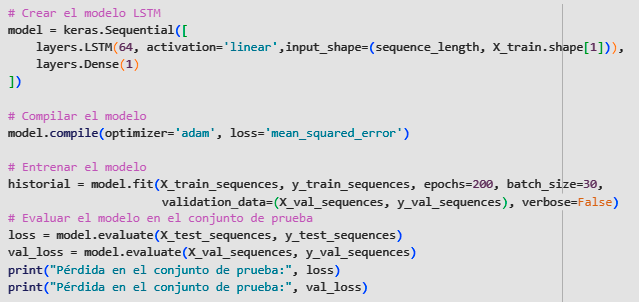
\includegraphics[scale=0.80]{./arqui1ie.png}
    \caption{Codigo de la estructura del LSTM datos de prueba 1.}
    \label{fig:arqui1ie}
  \end{center}
\end{figure}

El código presentado (Figura \ref{fig:arqui1ie}) es un ejemplo de construcción,
entrenamiento y evaluación de un modelo de red neuronal recurrente LSTM para un
problema de regresión. Se inicia con la definición del modelo, que consta de
una capa LSTM y una capa densa, seguido de la compilación con el optimizador
Adam y la métrica de pérdida de error cuadrático medio. El modelo se entrena
durante 200 épocas con lotes de tamaño 30, utilizando datos de entrenamiento y
validación. Luego se evalúa en un conjunto de prueba independiente y se calcula
la pérdida en el conjunto de validación para supervisar el rendimiento del
modelo. Las pérdidas resultantes se imprimen como indicadores de la calidad de
las predicciones del modelo en diferentes conjuntos de datos.

\begin{figure}[H]
  \begin{center}
    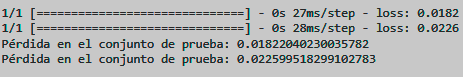
\includegraphics[scale=0.80]{./res1i.png}
    \caption{Rendimiento de datos de prueba 1.}
    \label{fig:rend1}
  \end{center}
\end{figure}

\textbf{27ms/step y 28ms/step:} Estas cifras (Figura \ref{fig:rend1}) indican el tiempo promedio que le toma al modelo procesar una iteración o paso de entrenamiento (epoch). En este caso, el modelo tarda aproximadamente 27-28 milisegundos en completar cada paso de entrenamiento. Este valor es útil para evaluar la eficiencia computacional del entrenamiento del modelo.

\vspace{1\baselineskip}
\textbf{loss: 0.0182 y loss: 0.0226:} Estos valores de la (Figura \ref{fig:rend1}) representan la pérdida (loss) del modelo en los datos de entrenamiento en dos momentos diferentes del entrenamiento. La pérdida es una medida que indica cuán diferente son las predicciones del modelo de los valores reales en los datos de entrenamiento. En este contexto, una pérdida de 0.0182 y 0.0226 sugiere que el modelo está haciendo buenas predicciones en los datos de entrenamiento, con 0.0182 siendo un valor ligeramente mejor (menos pérdida) que 0.0226. Sin embargo, es importante recordar que estos valores solo representan el rendimiento del modelo en los datos de entrenamiento y no necesariamente reflejan su capacidad para generalizar en datos no vistos, como el conjunto de prueba.

\begin{figure}[H]
  \begin{center}
    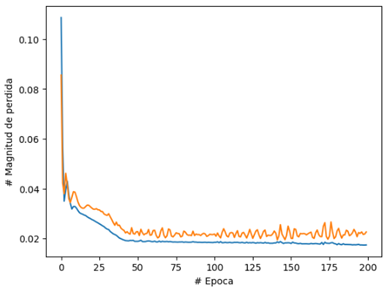
\includegraphics[scale=0.80]{./imagenlstm1.png}
    \caption{Grafico de predicción LSTM prueba 1}
    \label{fig:res2}
  \end{center}
\end{figure}

\vspace{1\baselineskip}
\textbf{Conjunto de prueba 2:}
\begin{itemize}
  \item División del conjunto de datos: 70\% train, 15\% validation, 15\% test
  \item Optimizador: Adam (learning\_rate=0.001)
  \item Pérdida: mean\_squared\_error
  \item Épocas: [50, 100, 200]
  \item Tamaño de lotes: [5, 10, 15]
  \item Estructura de red: 1 capa oculta con [32, 64, 128] neuronas
  \item Función de activación: relu
\end{itemize}

\begin{figure}[H]
  \begin{center}
    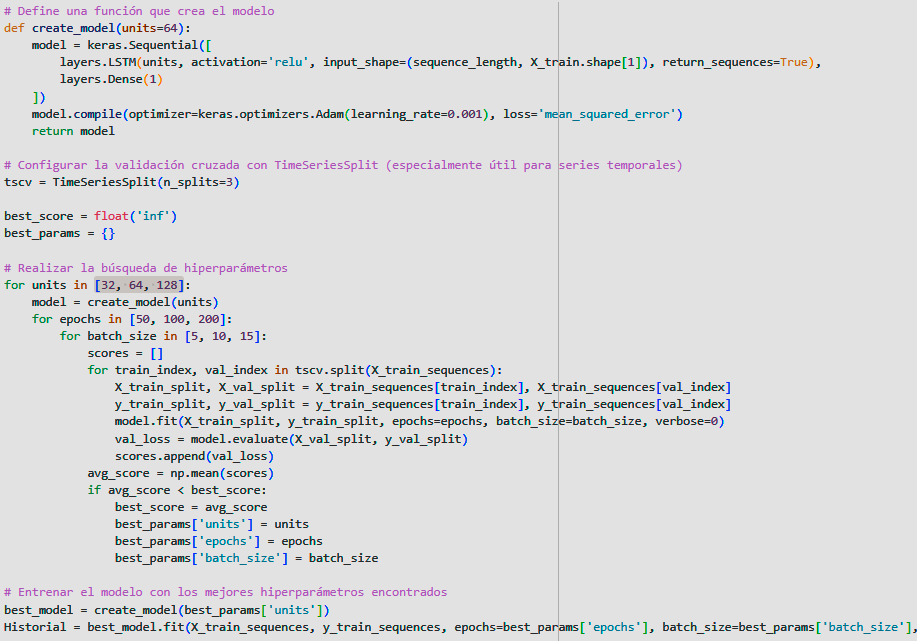
\includegraphics[scale=0.50]{./arqui2i.png}
    \caption{Codigo de la estructura del LSTM datos de prueba 2.}
    \label{fig:arqui2i}
  \end{center}
\end{figure}

El código (Figura \ref{fig:arqui2i}) presenta un proceso de búsqueda de
hiperparámetros para un modelo LSTM en datos de series temporales. Se definen
diferentes configuraciones de modelos con variaciones en el número de unidades
LSTM, épocas de entrenamiento y tamaño de lote.

\vspace{1\baselineskip}
Estos modelos se evalúan en un esquema de validación cruzada específico para series temporales, y se promedian las puntuaciones de rendimiento en las
divisiones de validación.

\vspace{1\baselineskip}
Los valores de hiperparámetros que generan la mejor puntuación se almacenan en best\_params.

\vspace{1\baselineskip}
Luego, se crea un modelo con estos hiperparámetros óptimos y se entrena en todo el conjunto de datos de entrenamiento.

\vspace{1\baselineskip}
Esta metodología busca encontrar la configuración de modelo que se ajuste mejor a los datos de series temporales, garantizando que el modelo sea robusto y pueda generalizar efectivamente a datos futuros.

\begin{figure}[H]
  \begin{center}
    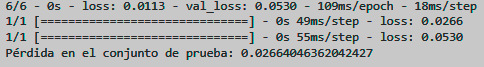
\includegraphics[scale=0.80]{./res2i.png}
    \caption{Rendimiento de datos de prueba 2.}
    \label{fig:res2}
  \end{center}
\end{figure}

En el contexto de un modelo LSTM entrenado en series temporales, los valores proporcionados representan métricas clave para evaluar su desempeño (Figura \ref{fig:res2}). 6/6 indica que se han completado seis épocas de entrenamiento,
mientras que 0s no especifica el tiempo transcurrido. La perdida (loss) de 0.0113 en el conjunto de entrenamiento señala un buen ajuste del modelo a los datos de entrenamiento, mientras que la val\_loss de 0.0530 en el conjunto de validación es ligeramente más alta, lo que sugiere que el modelo podría tener dificultades
para generalizar. Los tiempos en milisegundos por época y por paso (109ms/epoch y 18ms/step) reflejan la eficiencia de entrenamiento del modelo. En resumen, estas métricas ofrecen información sobre la capacidad del modelo para aprender
de los datos de entrenamiento y su habilidad para generalizar efectivamente a datos no vistos en el conjunto de validación, lo que es crucial en aplicaciones de series temporales.

\begin{figure}[H]
  \begin{center}
    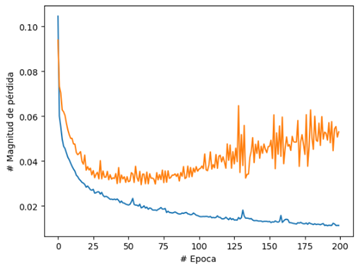
\includegraphics[scale=0.80]{./Imagenlstm2.png}
    \caption{Grafico de predicción LSTM prueba 2}
    \label{fig:res2}
  \end{center}
\end{figure}

\section{Prototipo del sistema}

El sistema web se desarrollará utilizando una combinación de tecnologías, que incluye PHP para la lógica del servidor, JavaScript para la interactividad y dinamismo en el lado del cliente, y HTML y CSS para la estructura y el diseño de la interfaz \cite{nixon2014learning}. Esta elección de tecnologías permite la creación de una aplicación web versátil y receptiva, que ofrece una experiencia de usuario intuitiva y eficiente, al tiempo que garantiza un sólido procesamiento en el servidor para gestionar las diversas funcionalidades del sistema.

\vspace{1\baselineskip}
El nuevo modelo debe garantizar el abastecimiento oportuno de productos sin
incurrir en sobre stock, minimizando el costo de inventario y facilitando el trabajo del área de compras. Para esto se propone diseñar y codificar una aplicación web que realice estas actividades, sin que los analistas deban realizar cálculo matemáticos complejos.


\vspace{1\baselineskip}
\textbf{Levantamiento de requisitos}

Importancia de la selección de una buena técnica de levantamiento de requerimientos 
Una técnica, es una serie de pasos documentados que van de la mano con unas reglas para su uso y criterios para verificar su corrección. Una técnica usualmente aplica a un proceso en el
modelo de procesos. Algunas veces, dicha técnica incluye una notación y/o una herramienta asociada \cite{mejia2009tecnicas}.

\vspace{1\baselineskip}
\textbf{Requisitos del sistema}
 \begin{itemize}

  \item Gestión de productos: 
  
  El sistema debe permitir la creación, modificación y eliminación de productos, incluyendo detalles como nombre.

  \item Órdenes de compra: 
  
  El sistema debe permitir la creación de órdenes de compra, especificando los productos y las cantidades.

  \item Órdenes de venta:
  
  Debe ofrecer la capacidad de crear órdenes de venta para registrar las transacciones, especificando los productos, las cantidades.
  
  \item Generación de informe: 
  
  Capaz de generar informes sobre las predicciones de los productos.
  
 \end{itemize}

 En el contexto de esta tesis, las entrevistas se utilizaron como una técnica esencial para la recolección de datos y la comprensión de los requerimientos del sistema.

 \vspace{1\baselineskip}
 Las órdenes de compra son vitales para registrar las adquisiciones de insumos, ya que nos permiten especificar los productos y sus cantidades. Asimismo, las órdenes de venta son esenciales para el registro de las ventas de productos finales, lo que proporciona un seguimiento preciso de las transacciones.

 \vspace{1\baselineskip}
La generación de informes cobra importancia para analizar y predecir el comportamiento de los productos, permitiéndonos realizar ajustes necesarios en nuestras predicciones. En resumen, estos requisitos se originaron directamente de la necesidad de abordar eficazmente la problemática de la gestión de insumos gastronómicos y garantizar un funcionamiento óptimo del sistema.
 
\vspace{1\baselineskip}
 El anexo de la tesis se convierte en un recurso valioso para aquellos lectores interesados en explorar en profundidad tanto la investigación cualitativa realizada a través de la entrevista como los aspectos técnicos y prácticos del prototipo desarrollado. Proporciona una visión completa de los dos componentes críticos de este trabajo: la obtención de requerimientos a través de entrevistas y la implementación técnica del sistema prototipo.


 
